\subsection{Dependence of $\rho_{max}$ and $n$ on Eigenvalue}
\label{subsec:DependenceOnEigenvalue}
\fxnote{include e.g. a section called "1 electron case" or smt similar}
For a single electron moving in a three-dimensional harmonic oscillator potential, the analytical solution for first three eigenvalues to the rewritten Schrödinger's equation 
\fxnote{eq. ref to nature eq} 
is $\lambda_0 = 3$, $\lambda_1 = 7$, and $\lambda_2 = 11$, for  $l=0$.
\fxnote{ref. to project description}

In the code given in ?? the two parameters $\rho_{max}$ and $n$ can be modified to give a more or less accurate numerical solution to the problem.
If not considering the computational time, limit in memory, and round-off errors, the obvious \fxnote{mest fordelagtige} choice of $\rho_{max}$ and $n$ would be to make both numbers infinite. 
This is, however, not a realistic possibility, and this sections is therefore dedicated to find (discuss) on the optimal choices for $\rho_{max}$ and $n$ to obtain acceptable values for the eigenvalues of \fxnote{eqref}.

Changing $\rho_{max}$ causes the interval $[\rho_{min}, \rho_{max}]$, in which the wave function is considered, to change. 
Since the wave function goes to zero as the distance goes to infinity, it is acceptable to neglect the contribution from some $\rho_{max}$. 
It is a \fxnote{fordel} to decrease $\rho_{max}$ and hence making the interval smaller, in the sense that a smaller $n$ then is needed to create a sufficient step length and ultimately a good enough "resolution". 
However, if this $\rho_{max}$ is too close to $\rho_{min}$ the neglected part can actually not be neglected, if an acceptable result is wished for. 

In the figure below, the dependence of different integer valued $\rho_{max}$ on the three first eigenvalues gained by the algorithm described in \fxnote{sec ref} is plotted for $n=100$. 
\fxnote{comment on, why we only have integer $\rho_max$}
\begin{figure}[H]
	\centering
	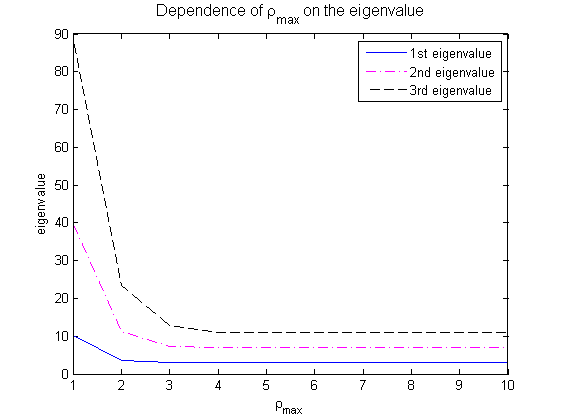
\includegraphics[width=0.75\textwidth]{Figures/rho_maxOnEigenvalue.png}
	\caption{Awesome caption}
	\label{fig:DependenceOnEigenvalue1}
\end{figure}
From the figure that if $\rho_{max} < 3$ the eigenvalues are varying dramatically.
This happens due to neglection ?? of strongly contributing parts of the eigenfunction. 
\fxnote{is this ok??}
\fxnote{comment on the flat part!!}
The $\rho_{max}$ that, with $n=100$, gives the most accurate result for all three of the first eigenvalues is $\rho_{max} = 5$. 
Since this $\rho_{max}$ gives the most accurate result for a relatively small $n$, this is chosen as the optimal $\rho_{max}$ in this and the following sections for this specific problem. 

With this $\rho_{max}$, we wish to find the number of $n$ that gives the first three eigenvalues with four leading digits. 
This optimal $n$ is found by steady increment of $n$, as seen in \fxnote{figref below}.
\begin{figure}[H]
	\centering
	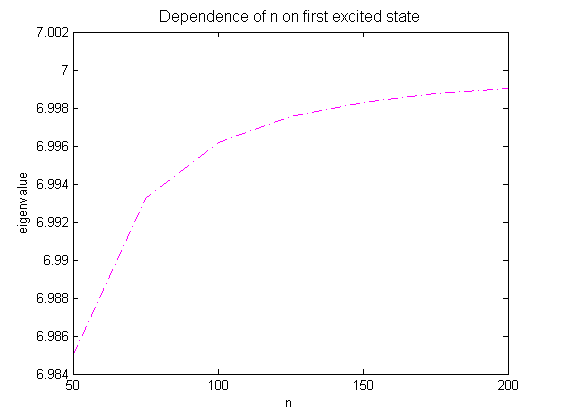
\includegraphics[width=0.75\textwidth]{Figures/MatrixSizeOnEigenvalue_2state.png}
	\caption{Awesome caption}
	\label{fig:DependenceOnEigenvalue2}
\end{figure}
The eigenvalue of the first exited is seen to be asymptotic to the analytical solution $\lambda_1 = 7$, and at a matrix size of $n=200$,  the eigenvalue of the first exited state has the numerical solution $6.99904$. 
This yields an accuracy up to four leading digits, which is also found to be the case for the ground state and the third eigenstate.
Hence, the optimal $\rho_{max}$ and $n$ is $5$ and $200$, respectively. 
